% !Mode:: "TeX:UTF-8"
% A4宽度 8.27 inches = 210.058 mm
% A4高度 11.69 inches = 296.926 mm
% 上左边距 > 25 mm = 0.984 inches
% 下右边距 > 20 mm = 0.787 inches
% 上边距 1.023 inches = 28 mm
% 左边距 1.3 inches = 33 mm
% 下边距 0.866 inches = 22 mm
% 右边距 0.984 inches = 25 mm
% 页眉页脚高度 1.18 inches = 29.972 mm
% 210.058 - 33 - 25 = 152.058 mm
% 296.926 - 22 - 28 = 246.926 mm
%\usepackage[a4paper,text={1\textbf{•}52.058 true mm,246.926 true mm},top= 28 true mm,left=33 true mm,head=10 true mm,headsep=6.5 true mm,foot=8 true mm]{geometry}
%\newgeometry{top= 28 true mm,bottom=22 true mm,left=13 true mm,right=25 true mm,head=10 true mm,headsep=6.5 true mm,foot=8 true mm}
%\newgeometry{text={172.058 true mm,246.926 true mm},top= 28 true mm,left=13 true mm,head=10 true mm,headsep=6.5 true mm,foot=8 true mm}
% 设置该选项为空是为了不让目录中显示页码
\titlecontents{chapter}[2em]{\vspace{.2\baselineskip}\bf\xiaosi\song}%
             {\prechaptername\zhnumber{\thecontentslabel}\postchaptername\qquad}{}{}             
\setcounter{page}{1}       % 如果需要从该页开始从 1 开始编页,则取消该注释
\markboth{外文资料}{外文资料}
\addcontentsline{toc}{chapter}{外文资料}
\fancypagestyle{plain}{                              
    \fancyhf{}
    \fancyhead[L]{\song\wuhao 附录}
    \fancyhead[R]{\song\wuhao 外文资料}           
    \fancyfoot[C]{\song\xiaowu~\thepage~}
    \renewcommand{\headrulewidth}{0.5pt}
    \renewcommand{\footrulewidth}{0pt}
}
\pagestyle{plain}
\fancyhf{}
\fancyhead[L]{\song\wuhao 附录}
\fancyhead[R]{\song\wuhao 外文资料}           
\fancyfoot[C]{\song\xiaowu~\thepage~}
\renewcommand{\headrulewidth}{0.5pt}
\renewcommand{\footrulewidth}{0pt}
\chapter*{\centering\sanhao\hei 外文资料}

\begin{figure}[htbp] 
\centering
\vspace{-22pt}
\noindent\hspace{-1.5em}\makebox[\textwidth][l] {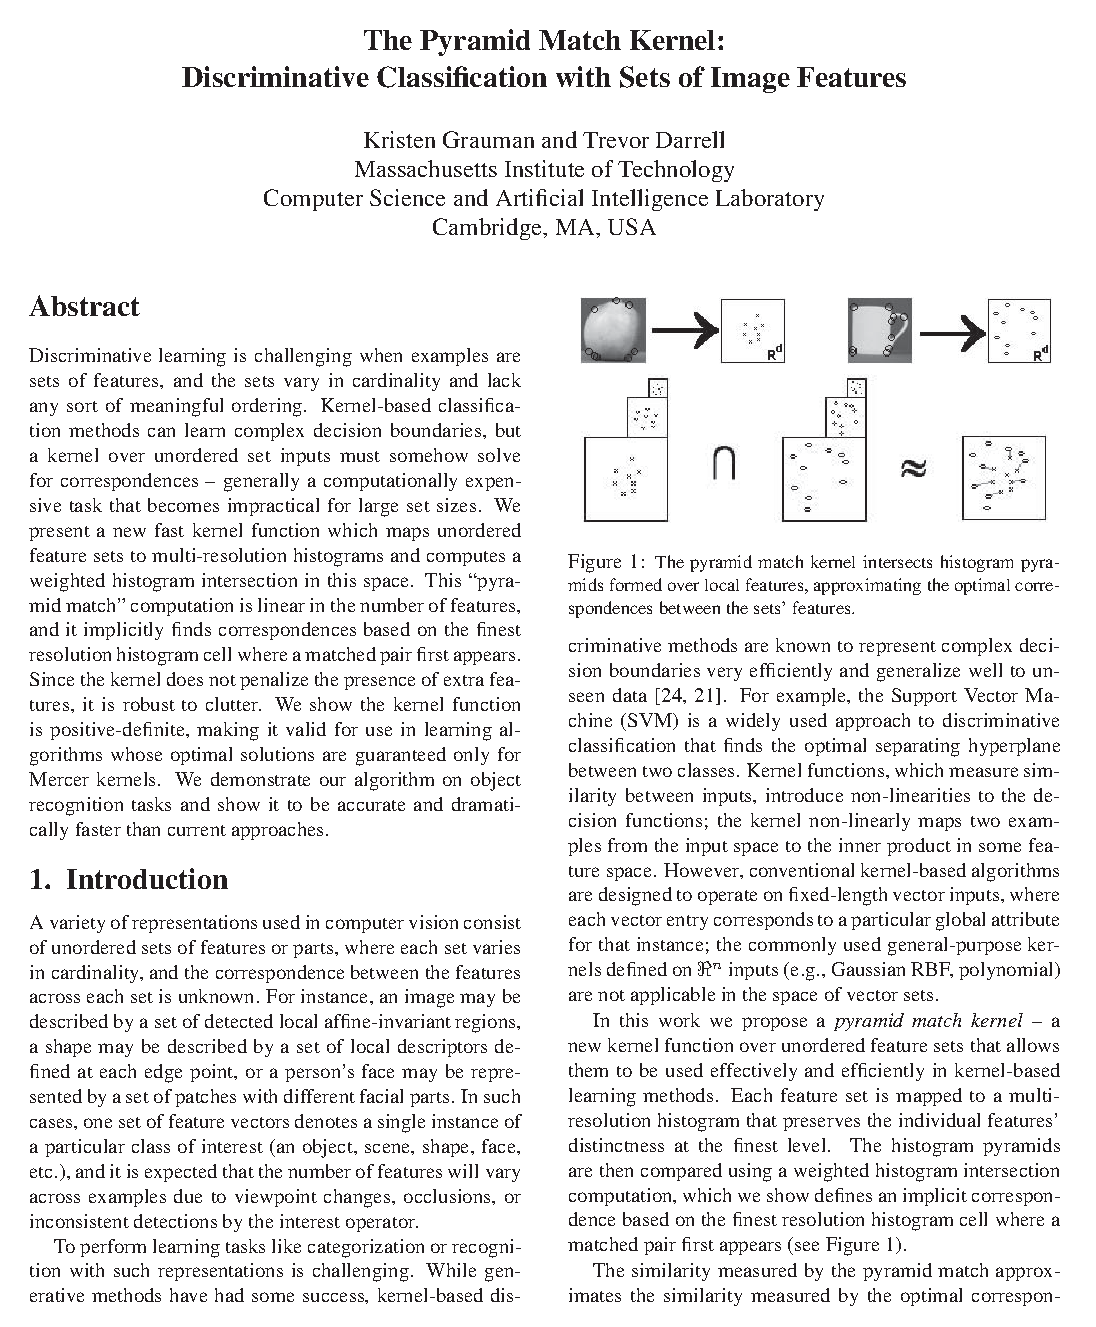
\includegraphics[width=1.08\textwidth]{figures/papers_1}}
\end{figure}
\begin{figure}[htbp] 
\centering
\noindent\hspace{-1.5em}\makebox[\textwidth][l] {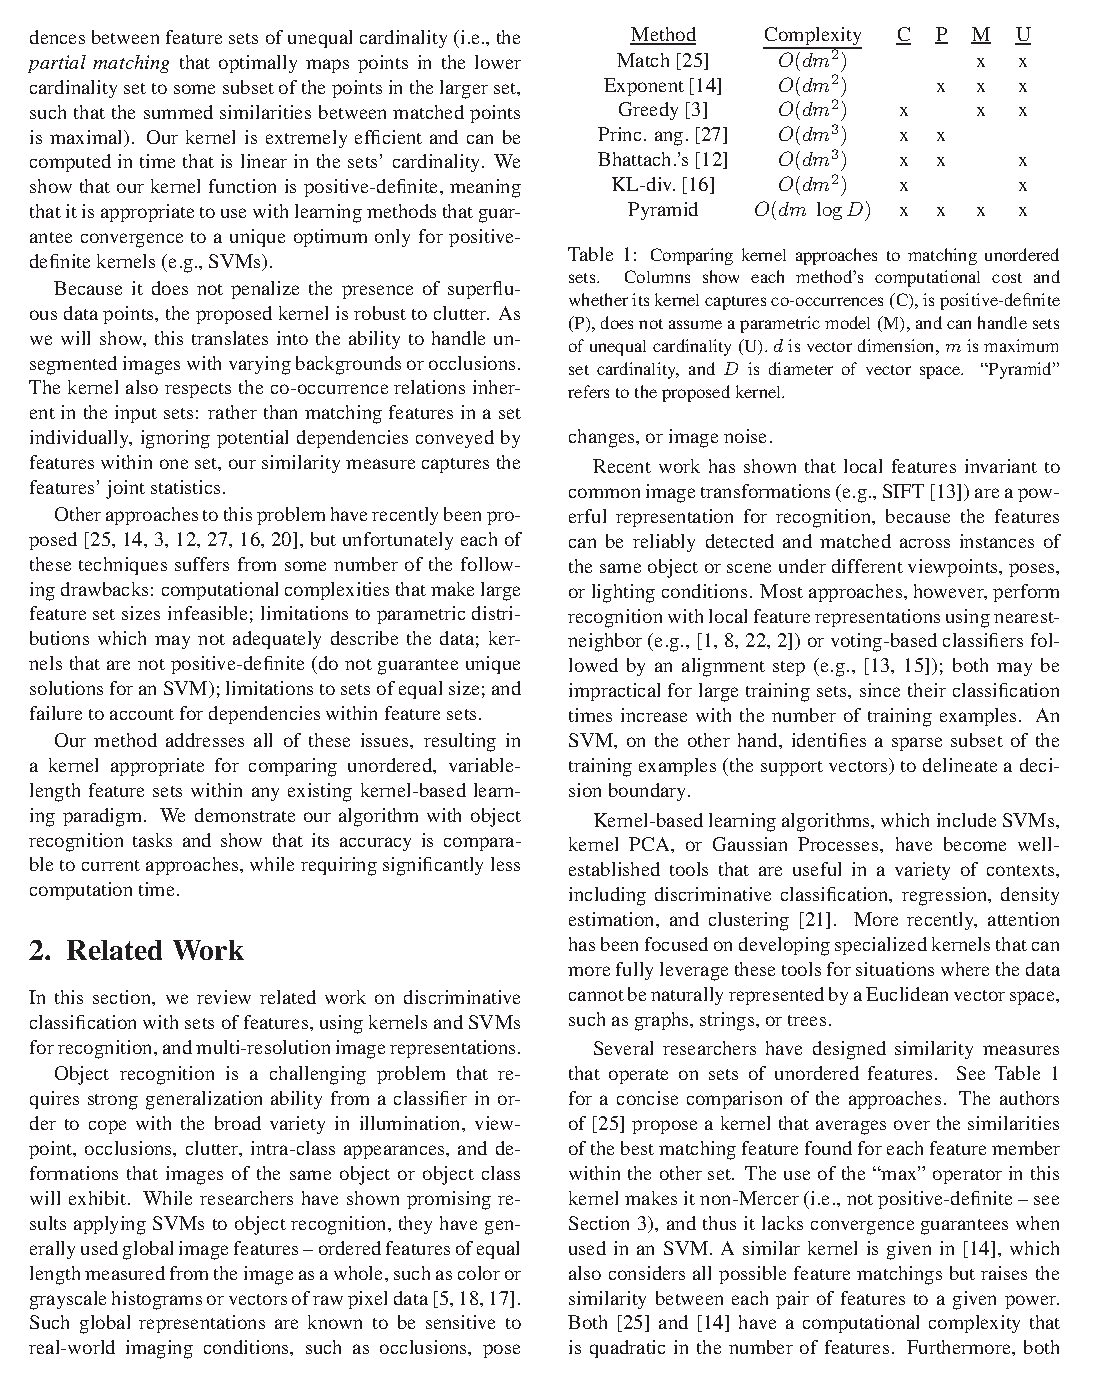
\includegraphics[width=1.08\textwidth]{figures/papers_2}}
\end{figure}

%\restoregeometry
%In this work, we propose an efficient method to automatically learn groupings over sets of unordered local features by embedding the sets into a space where they cluster according to their partial-match correspondences. Each image is decomposed into a set of local feature descriptors. Then every set is treated as a node in a graph, where an edge between two nodes (sets) is weighted according to how well some subset of the two sets features may be put into correspondence, with correspondence quality determined by descriptor similarity. A spectral clustering algorithm is then applied to the graph's affinity matrix to produce an initial set of image groupings. In an (optional) semi-supervised paradigm, we allow the user to select pairwise constraints between some number of input images, where constraints are in the form of "must-group" or "cannot-group" specifications. The affinity matrix is then modified to incorporate the user-supplied groupings prior to the spectral clustering step.
%
%
%Spectral clustering on approximate partial-match similarity scores is efficient and produces clusters that coarsely group distinct object classes. To improve specificity, and to develop a predictive classifier that can label unseen images, we develop a method to find prototypical examples in each cluster that are more likely to be class inliers, and then use these prototypes to train a predictive model.
%
%
%We detect prototype examples by examining the pattern of partial match correspondences within a cluster. Outlier cluster members are identified as those images that cause most images within the cluster to contribute an inconsistent subset of features in a partial match. With the assumption that outlier images will be less likely to match the same features as the majority of inlier images, we re-weight intracluster matching scores under a per-image mask representing the image elements that were most likely to be in correspondence when matched to other examples in the cluster.
%
%...
